\chapter{Regulacja procesu}
	\label{ch:reg}
	
	\section{Implementacja NPL}
		\label{sec:NPL}
		NPL jest algorytmem regulacji predykcyjnym z Nieliniową predykcją i z linearyzacją oznacza to że do wyznaczania trajektori swobodnej (która zależy tylko od przeszłych sterowań) używamy nieliniowego modelu neuronowego:
		\begin{equation}
		\begin{tabular}{l}
		$y^0(k+1)=w20+w2*tanh(w10+w1*x(k))+dk$
		\end{tabular}
		\label{eq:NPL_y0}
		\end{equation}
		gdzie
		\begin{equation}
		\begin{tabular}{l}
		$dk = y(k)-y^M(k)$
		\end{tabular}
		\label{eq:dk}
		\end{equation}
		\begin{equation}
		\begin{tabular}{l}
		$x(k)=$ $\begin{bmatrix}u(min(k-\tau+n,k-1))\\u(min(k-\tau-1+n,k-1\\y(k-1+n)\\y(k-2+n)))\end{bmatrix}$
		\end{tabular}
		\label{eq:wesn}
		\end{equation}
		$n=$ ilość chwil w przyszłóść.
		Warto dodać, że we wzore \ref{eq:wesn} dla chwil czasu dalszych od $k$ zakłada się że $y(p>k)=y^0(p)$.\\
		Aby móc rozwiązać algorytm analitycznie dokonuje się linearyzacji predykcji wyjścia modelu w przyszłości. Współczynniki $b_3$,$b_4$,$a_1$,$a_2$ we wzorze
		\begin{equation}
		\begin{tabular}{l}
		$y(k)=b_3u(k-\tau=k-3)+b_4(k-\tau-1=k-4)-a_1y(k-1)-a_2y(k-2)$
		\end{tabular}
		\label{eq:NPL_wyjscielinear}
		\end{equation}
		otrzymuje się poprzez obliczenie pochodnej cząstkowej po odpowiednim wejściu modelu neuronowego. Mając obliczone współczynniki można użyć ich do wyznaczenia odpowiedzi skokowej ze wzoru
		\begin{equation}
		\begin{tabular}{l}
		$s_j(k)=\sum\limits_{i=1}^{min(j,n_B)}b_i(k)-\sum\limits_{i=1}^{min(j-1,n_A)s_{j-i}(k)}$
		\end{tabular}
		\label{eq:NPL_odpowiedzskok}
		\end{equation}
		których można użyć do wypełnienia macierzy dynamicznej.
		Na koniec można obliczyć optymalne przyszłe sterowania(przy zadanych horyzntach i współczynniku kary)
		\begin{equation}
		\begin{tabular}{l}
		$du=K*(y_{zad}-y^0)$
		\end{tabular}
		\label{eq:NPL_du}
		\end{equation}
		gdzie
		\begin{equation}
		\begin{tabular}{l}
		$K=(M'*M+\lambda I)^{-1}*M'$
		\end{tabular}
		\label{eq:NPL_du}
		\end{equation}
	
		
		
	\section{Strojenie NPL}
		\label{sec:stroj_NPL}
		Strojenie regulatora NPL rozpoczęliśmi od parametrów $N=10$, $N_u=2$ oraz $\lambda=1$. Przebieg dla tych wartości zaprezentowany jest ponieżej (rys. \ref{fig:NPL0}).
		
		\begin{figure}[h!]
			\centering
			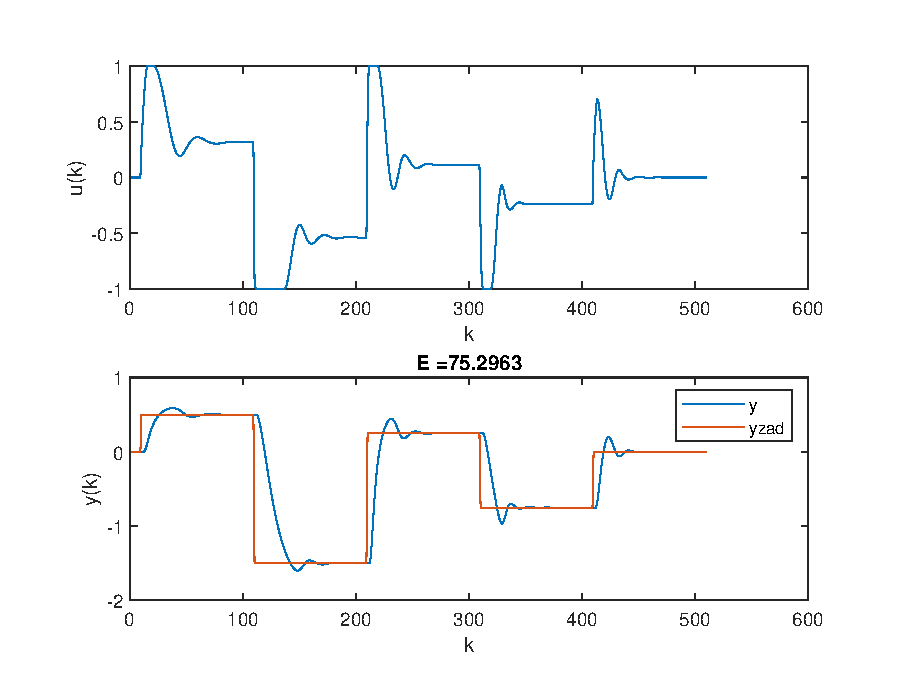
\includegraphics[width=\linewidth]{img/strojenieNPL_N_10_Nu_2_lam_1.eps}
			\caption{Działanie regulatora NPL z nastawami N=10, Nu=2, $\lambda$=1}
			\label{fig:NPL0}
		\end{figure}
		
		Postanowiliśmy zwiększać horyzont predykcji do czasu zmniejszania się wartości błędu i ogólnej jakości sterowania, najlepszą jakość udało nam się uzyskać dla $N=20$ (rys. \ref{fig:NPL1}).
		\begin{figure}[h!]
			\centering
			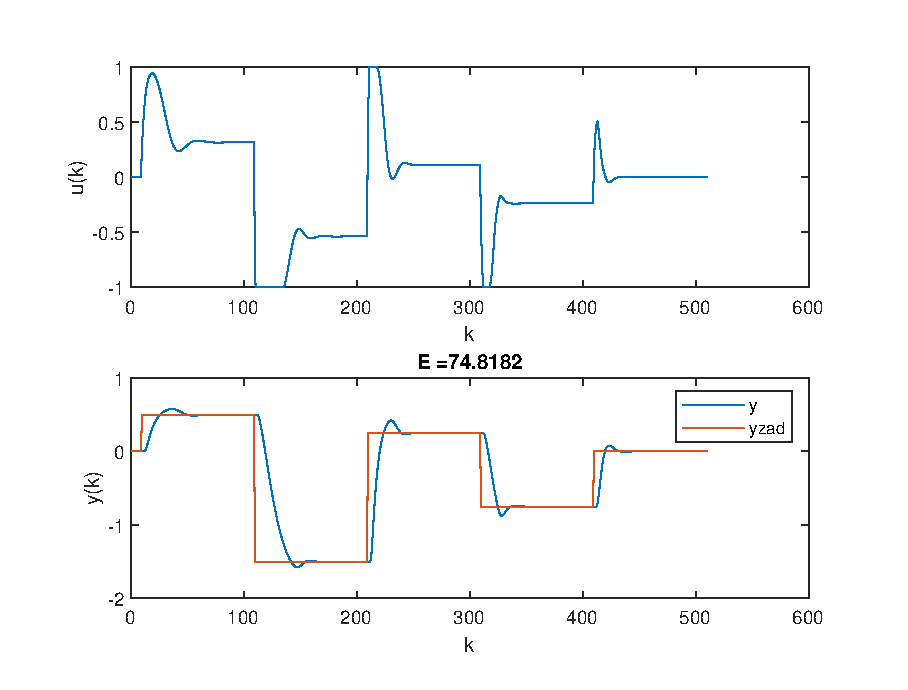
\includegraphics[width=\linewidth]{img/NPLN20.eps}
			\caption{Działanie regulatora NPL z nastawami N=20, Nu=2, $\lambda$=1}
			\label{fig:NPL1}
		\end{figure}
		
		Następnie postanowiliśmy dobrać horyzont sterowania. Niestety zarówno przy zwiększaniu jak i zmniejszaniu horyzunto jakość regulacji pogarszała się, co można zaobserwować na wykresach \ref{fig:NPL2} i \ref{fig:NPL3}.
		\begin{figure}[h!]
			\centering
			\includegraphics[width=\linewidth]{img/NPLNu1.eps}
			\caption{Działanie regulatora NPL z nastawami N=20, Nu=1, $\lambda$=1}
			\label{fig:NPL2}
		\end{figure}
		
		\begin{figure}[h!]
			\centering
			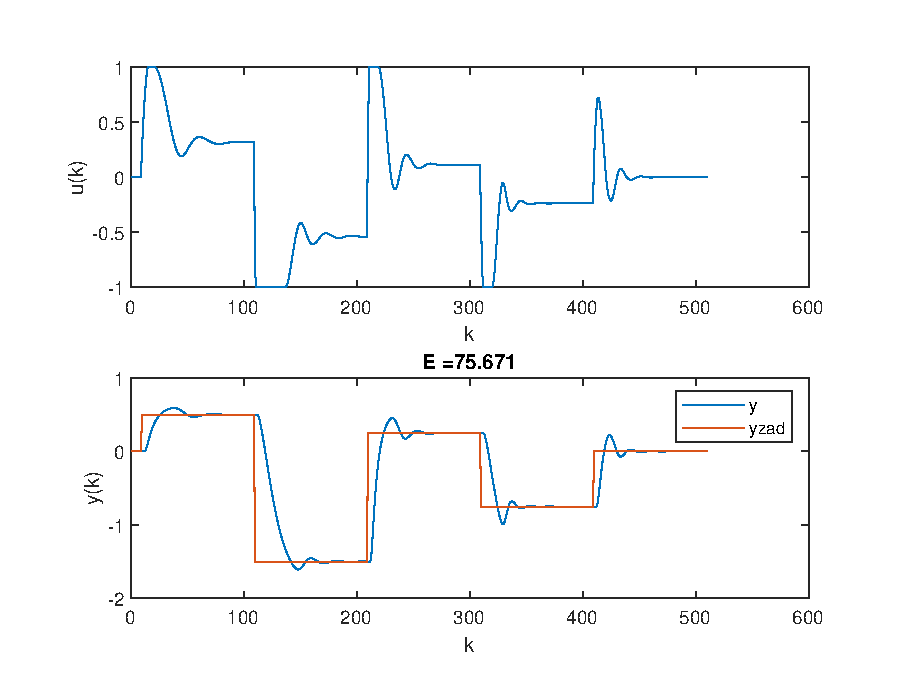
\includegraphics[width=\linewidth]{img/NPLNu3.eps}
			\caption{Działanie regulatora NPL z nastawami N=20, Nu=3, $\lambda$=1}
			\label{fig:NPL3}
		\end{figure}
		
		Mając dobrane $N$ oraz $N_u$ pozostało zbadać wpływ współczynnika $\lambda$. Po zwiększeniu o jeden dało się zaobserwować spadek oscylacji, wygładzenie sterowania ale spadek przeregulowania, niestety jednak wartość błędu liczonego ze wzoru \ref{eq:error} wzrosła, dlatego postanowiliśmy zostawić $\lambda$ przy obecnej wartości (rys. \ref{fig:NPL4}).
		\begin{figure}[h!]
			\centering
			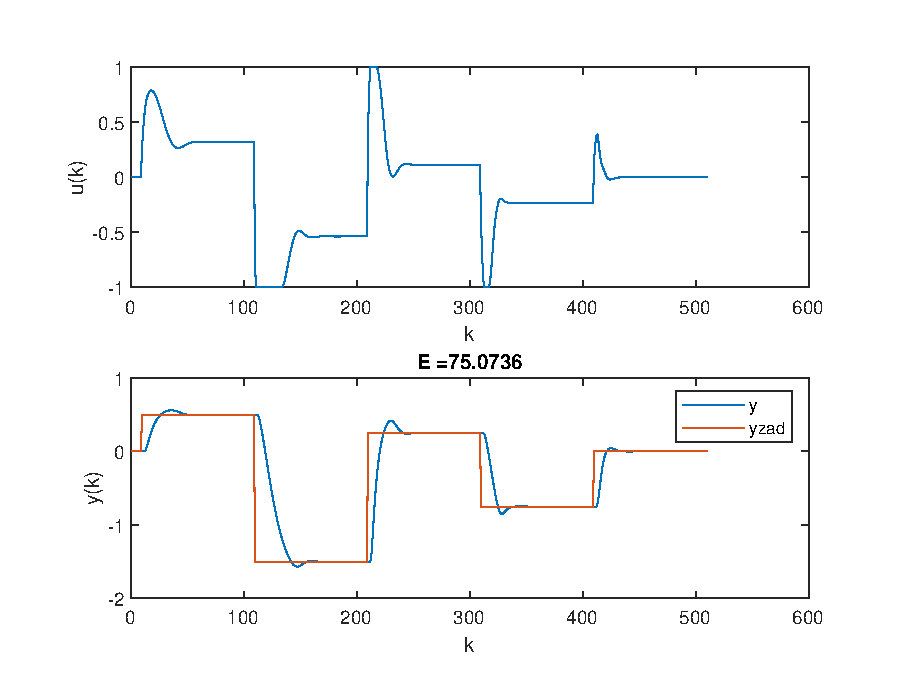
\includegraphics[width=\linewidth]{img/NPLlam2.eps}
			\caption{Działanie regulatora NPL z nastawami N=20, Nu=2, $\lambda$=2}
			\label{fig:NPL4}
		\end{figure}
		
		
	\section{GPC}
		\label{sec:GPC}
		Algorytm regulacji GPC, różni się tym od NPL, że na całym horyzocnie predykcji korzysta się z liniowego modelu wyznaczonego metodą najmniejszych kwadratów. Jak można było zauważyć z rys. \ref{fig:mnk} taki model nie gwarantuje najlepszego odwzorowania obiektu, przez co jak można się domyślać jakość regulacji również może być gorsza.
		Do wyznaczania sterowania w wersji analitycznej wyznacza predykcje wyjscia modelu $N$ chwil do przodu ze wzoru
		\begin{equation}
		\begin{tabular}{l}
		$y^0(k+n)=b_3u(min(k-3+n,k-1))+b_4u(min(k-4+n),k-1)-a_1y(k-1+n)-a_2y(k-2+n)$
		\end{tabular}
		\label{eq:NPL_odpowiedzskok}
		\end{equation}
		oraz analogicznie do wzoru \ref{eq:NPL_y0} $y(p>k)=y^0(p)$. Macierz dynamiczna jest stała i wyznaczana przy użyciu odpowiedzi skokowej ze wzoru \ref{eq:NPL_odpowiedzskok}. Na wykresie poniżej można zauważyć, że jakość regulacji w istocie pozostawia wiele do życzenia (rys \ref{fig:GPC}).
		
		\begin{figure}[h!]
			\centering
			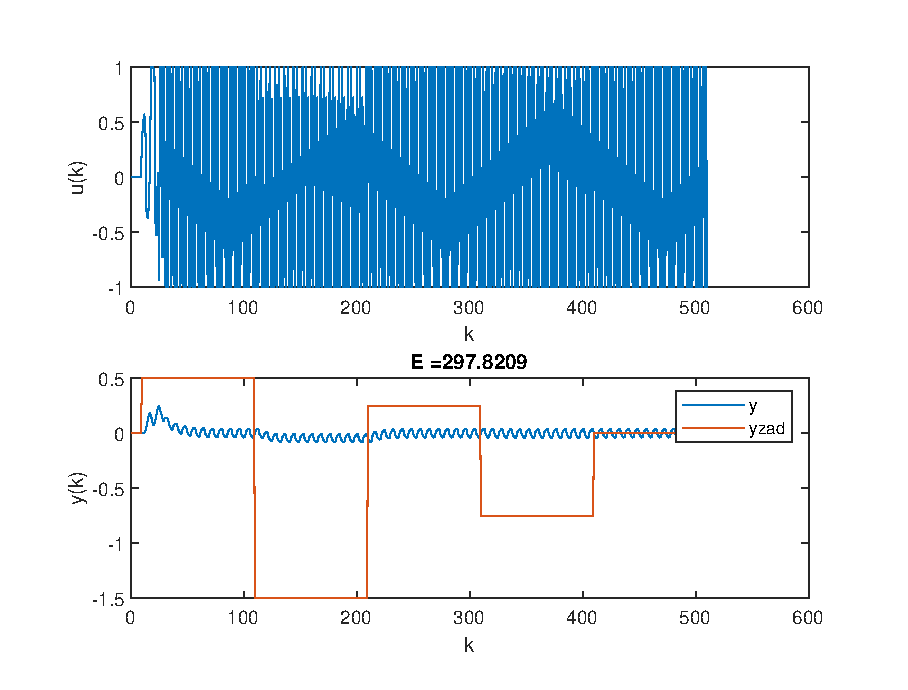
\includegraphics[width=\linewidth]{img/GPC.eps}
			\caption{Działanie regulatora GPC z nastawami N=20, Nu=2, $\lambda$=2}
			\label{fig:GPC}
		\end{figure}
	
		Należy wziąć pod uwagę, że przez silną nieliniowość obiektu, liniowy algorytm GPC może generować duże sterowania, które po nałożeniu ograniczeń wprowadzą obiekt w stałe oscylacje. Można temu zapobiec poprzez zwiększenie współczynnika $\lambda$ o parę rzędów wielkości.
		\begin{figure}[h!]
			\centering
			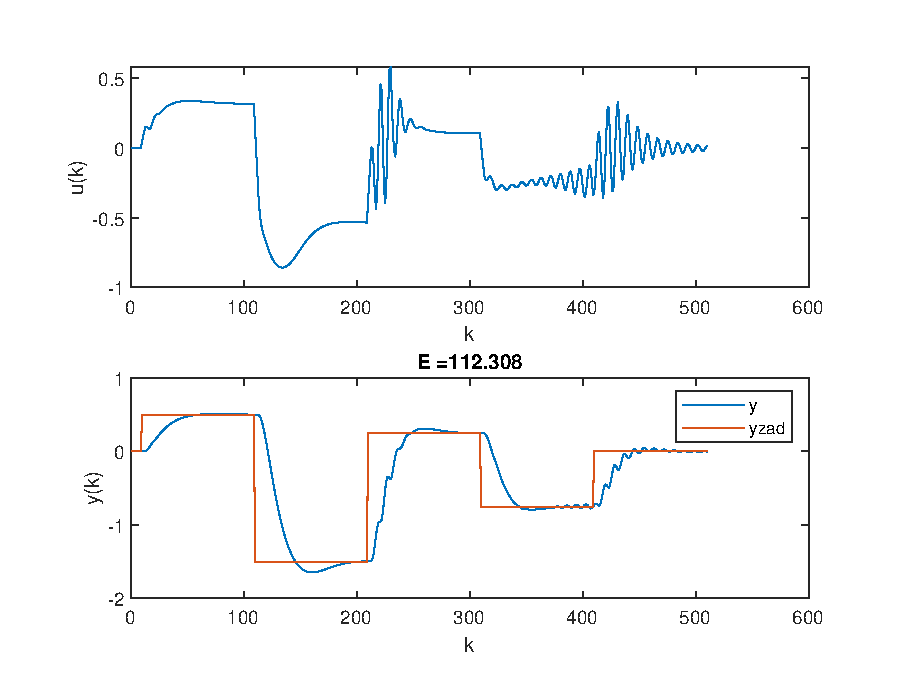
\includegraphics[width=\linewidth]{img/GPC100.eps}
			\caption{Działanie regulatora GPC z nastawami N=20, Nu=2, $\lambda$=100}
			\label{fig:GPC100}
		\end{figure}
		Na rys. \ref{fig:GPC100} można zobaczyć, że jakość regulacji polepszyła się, lecz mimo to sterowanie wciąż jest zbyt ostre, a czas regulacji wolniejszy niż w przypadku NPL.